\chapter{Method}
\begin{itemize}
\item Introduce requirements
\item Need disentangled latent space
\item Explain degree of freedom here (disentangled filters, or disentangled neurons, or something else?)
\item Need to preserve spatial information for symbolic front-end
\end{itemize}

\label{ch:method}

%
%
%
%
%
\section{Latent Image}
\lipsum[2]
\subsection{Architecture}
\begin{figure}[H]
\centering
\captionsetup{justification=centering}
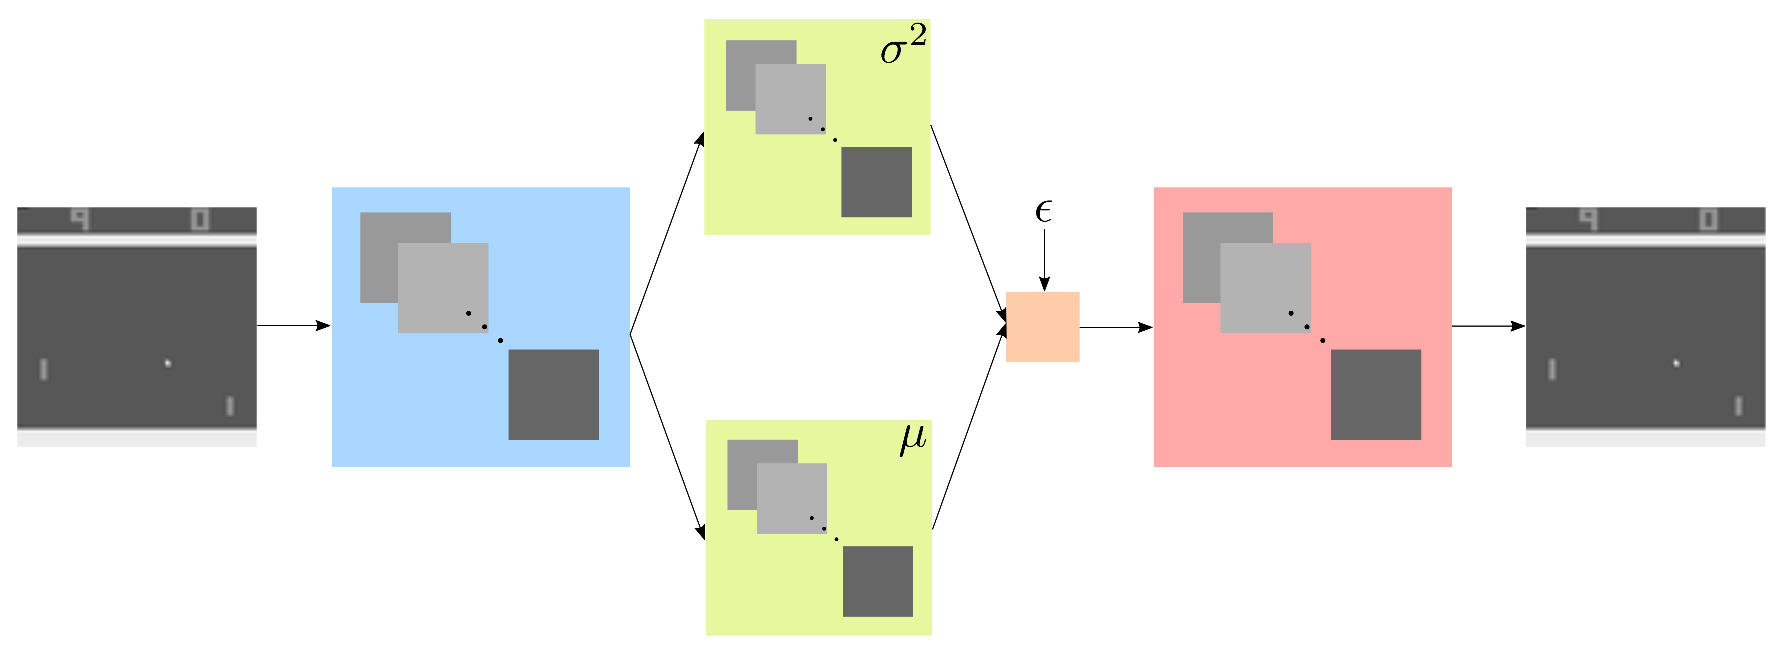
\includegraphics[scale=0.8]{methods/latent_image_architecture.eps}
\caption{Caption.}
\label{fig:latent_image_architecture}
\end{figure}

\subsection{Derivation}

%
%
%
%
%
\section{Decoupling Latent Variables Indiscriminately}
\lipsum[2]
\subsection{Architecture}
\begin{figure}[H]
\centering
\captionsetup{justification=centering}
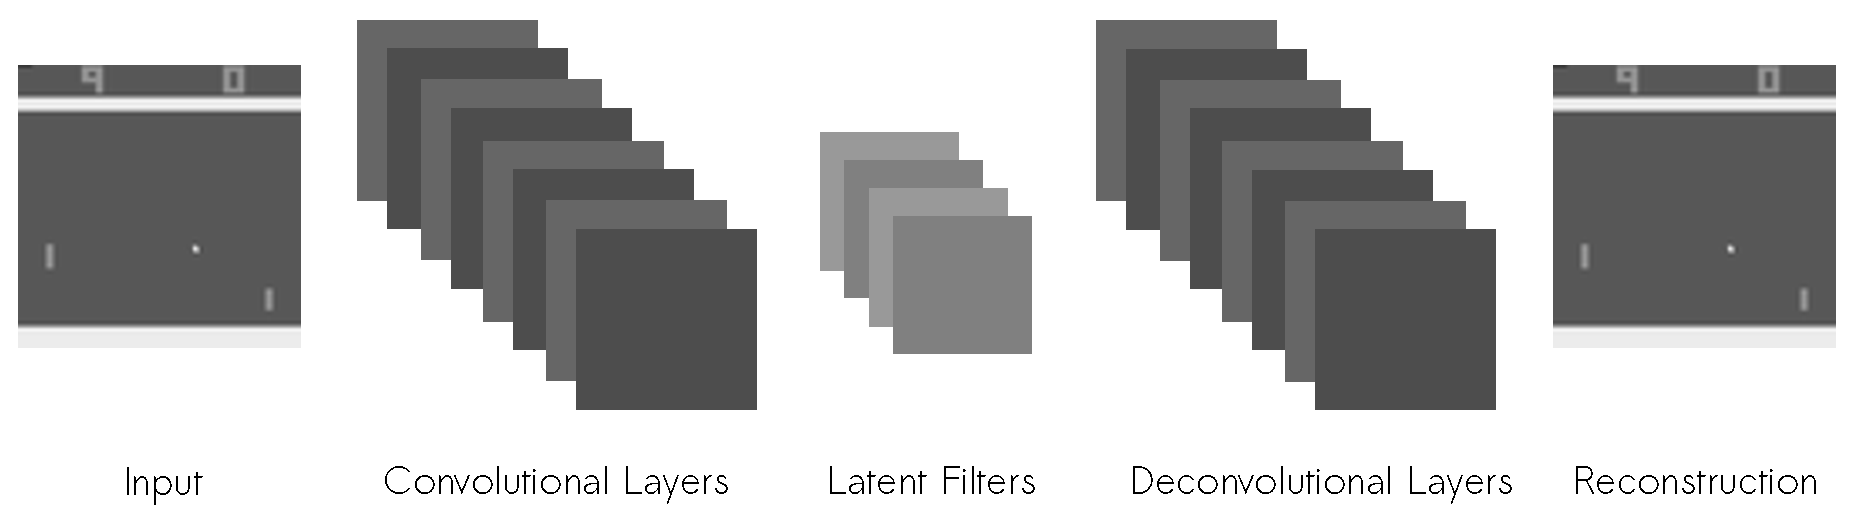
\includegraphics[scale=0.55]{methods/decoupling_indiscriminately.eps}
\caption{Caption.}
\label{fig:decoupling_indiscriminately}
\end{figure}

\begin{figure}[H]
\centering
\captionsetup{justification=centering}
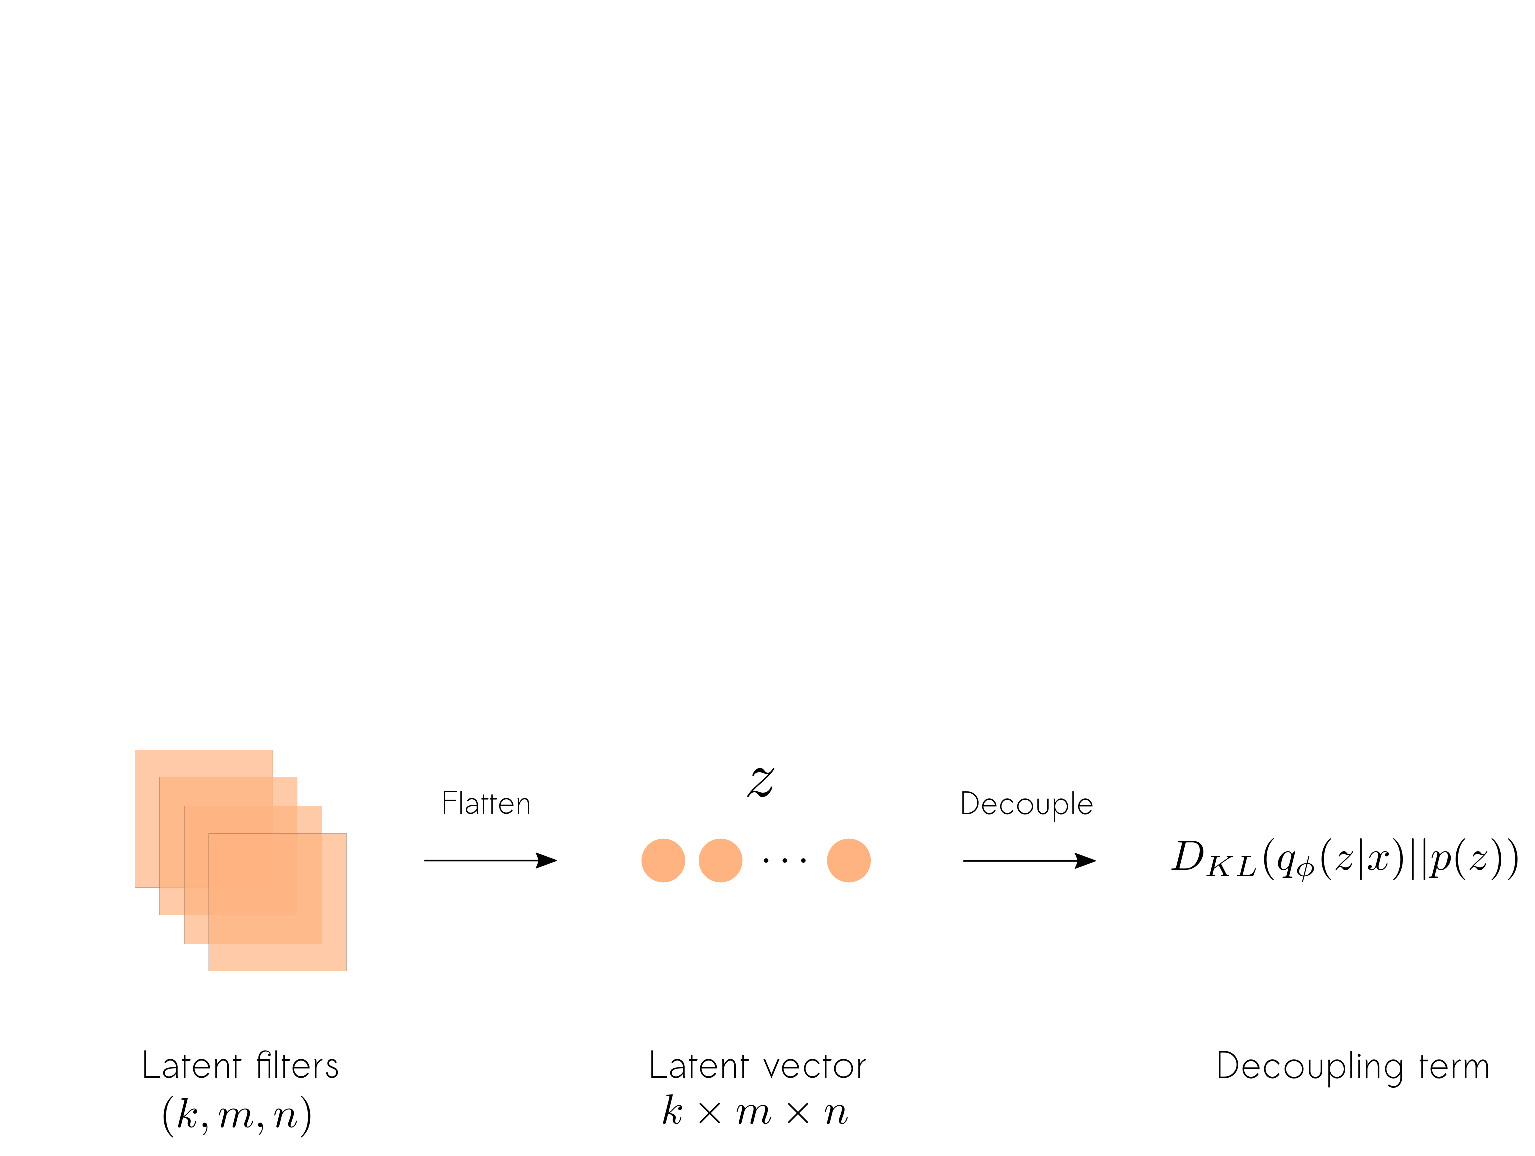
\includegraphics[scale=0.55]{methods/decoupling_indiscriminately_flattening_latent_space.eps}
\caption{Caption.}
\label{fig:decoupling_indiscriminately_flattening_latent_space}
\end{figure}

\subsection{Derivation}



%
%
%
%
%
\section{Decoupling Latent Filters Using Averages}
\lipsum[2]
\subsection{Architecture}
\begin{figure}[H]
\centering
\captionsetup{justification=centering}
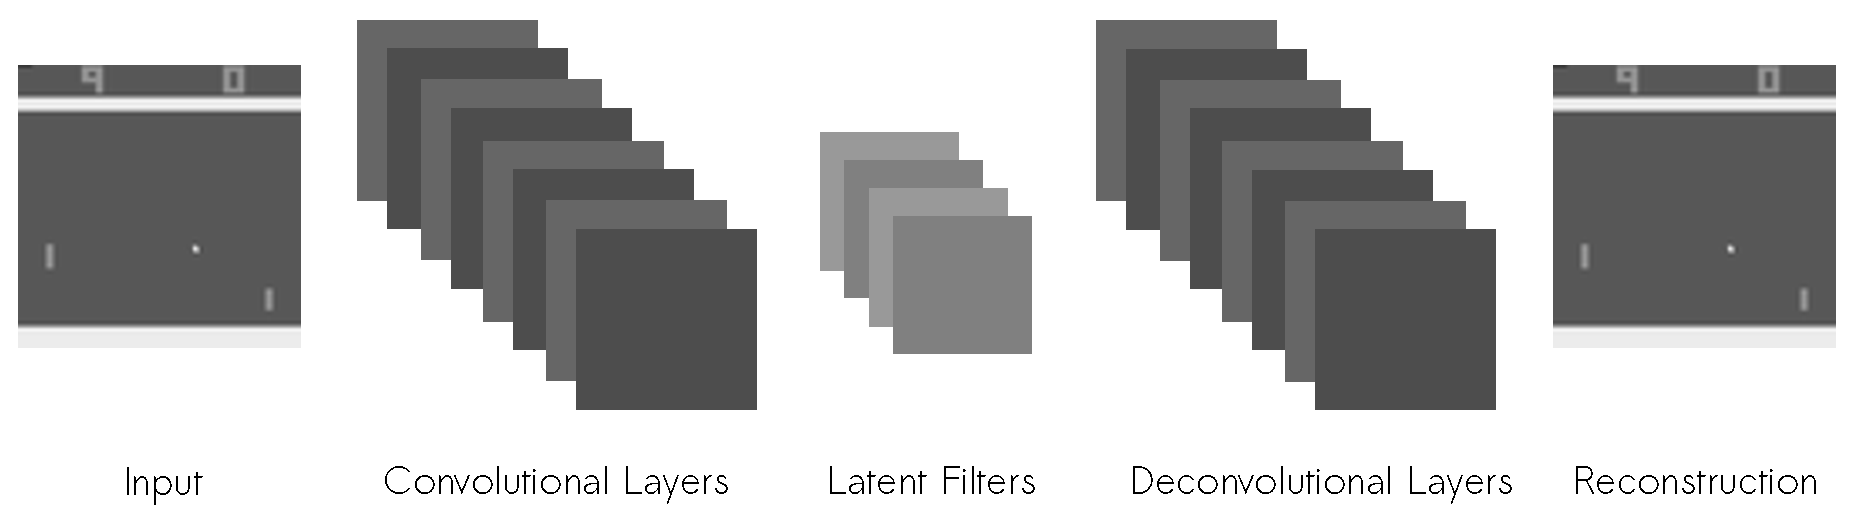
\includegraphics[scale=0.55]{methods/decoupling_indiscriminately.eps}
\caption{Caption.}
\label{fig:decoupling_indiscriminately}
\end{figure}

\begin{figure}[H]
\centering
\captionsetup{justification=centering}
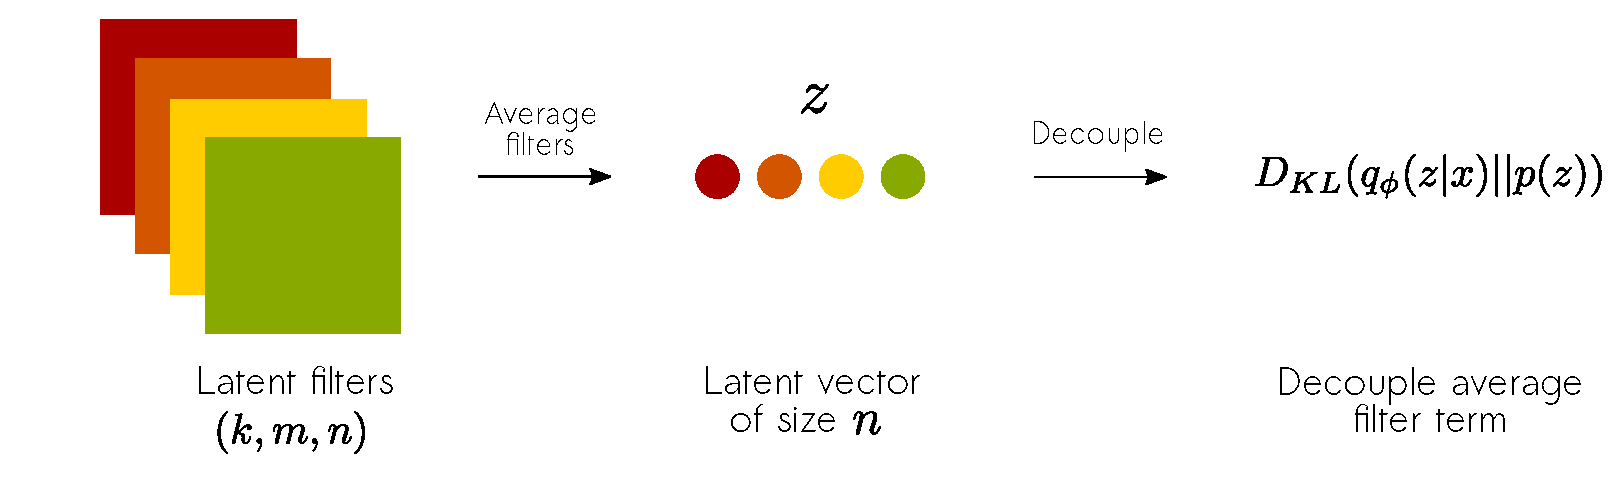
\includegraphics[scale=0.55]{methods/decoupling_averages_latent_space.eps}
\caption{Caption.}
\label{fig:decoupling_averages_latent_space}
\end{figure}

\subsection{Derivation}

%
%
%
%
%
\section{Decoupling Latent Filters Using Weighted-Averages}
\lipsum[2]
\subsection{Architecture}
\subsection{Derivation}

%
%
%
%
%
\section{Separating Colour Spaces}
\lipsum[2]
\subsection{Architecture}
\subsection{Derivation}

%
%
%
%
%
\section{Orthogonal Convolutions}
\lipsum[2]
\subsection{Architecture}
\subsection{Derivation}

%
%
%
%
%
\section{Winner Takes All}
\lipsum[2]
\subsection{Architecture}
\subsection{Derivation}

%
%
%
%
%
\section{Psuedo-Dense Latent Space}
\lipsum[2]
\subsection{Architecture}
\subsection{Derivation}
